\documentclass[12pt,titlepage]{article}

\usepackage{listings}

% Geometry
\usepackage{geometry}
\newgeometry{top=2.25cm,right=2cm,bottom=2.5cm,left=3cm}
% Graphics
\usepackage{graphicx}
\graphicspath{{images/}{../images/}}
% Times new roman package
\usepackage{mathptmx}
% Linespread of 1.5 as required by SIT
\linespread{1.5}
% URL
\usepackage{hyperref}
% Page rotation
\usepackage{pdflscape}
% CSV tables
\usepackage{csvsimple,booktabs,longtable}
% Define a command to read in CSVs (filename, caption, label)
\newcommand{\csvtable}[3]{
  \csvreader[
    longtable=ll|l,
    table head=
      \caption{#2}
      \label{#3}\\
      \toprule
      \bfseries From & \bfseries To & \bfseries Frequency \\
      \midrule
      \endfirsthead
      \caption*{Table \ref{#3} (\textit{continued from Page~\pageref{#3}}): #2}\\\toprule
      \bfseries From & \bfseries To & \bfseries Frequency \\
      \midrule
      \endhead
      \bottomrule
      \textit{Continued on next page...}
      \endfoot
      \bottomrule
      \endlastfoot
  ]{#1}{1=\From,2=\To, 3=\Frequency}{\From & \To & \Frequency}
}
% Define a command to import the dot figure
\newcommand{\dotfigure}[2]{
  \newpage
  \begin{figure}[p]
    \centering
    \includegraphics[width=\textwidth]{figs/digraphs/#1}
    \caption{#2. Refer to Table~\ref{tbl:#1} for frequency pattern interactions.}
    \label{fig:#1}
  \end{figure}
  \clearpage
  \newpage
}

\author{Alex Cummaudo \texttt{<ca@deakin.edu.au>}\\ Jake Renzella \texttt{<jake.renzella@deakin.edu.au>}\\
Deakin Software and Technology Innovation Laboratory\\School of Information Technology\\Deakin University, Australia}
\title{Hotel TULIP Web Server Data Analysis\\\normalsize{\bfseries Assignment 2 - SIT742 Modern Data Science}}

\begin{document}

\maketitle

\section*{Executive Summary}

This report summarises findings from a data exploration on the Hotel TULIP web server logs, recorded between the periods of August 2014 and August 2015. Each log contains one \textit{request}, or \textit{hit}, that lists fourteen attributes as described in the attached Data Dictionary spreadsheet. Publicly known client IP addresses were extracted from the MaxMind GeoIP2\footnote{See \url{http://dev.maxmind.com/geoip/geoip2/}.} dataset to analyse the location of requests (narrowed down to city). Additionally, user agent strings were parsed to analyse device and browser statistics using the Python \texttt{user-agents} library\footnote{See \url{https://pypi.python.org/pypi/user-agents}.}, thereby extrapolating demographics, usage trends, platform information, server performance, and security statistics from the raw logs provided in the dataset. Further details on the extraction of the data is provided in the source code attached in Appendix~\ref{apx:results}, and an interactive version of this file is published on \href{https://databricks-prod-cloudfront.cloud.databricks.com/public/4027ec902e239c93eaaa8714f173bcfc/7364378259770565/3552971541306612/8155742302574378/latest.html}{Databricks}.

\newpage

\tableofcontents\newpage
\listoffigures\newpage
\listoftables\newpage

\newpage
\section{Key Findings}

A list of key findings in the analysis are as thus:

\begin{itemize}
  \item Foo
\end{itemize}

\newpage
\section{Introduction}

Browsing patterns on the Hotel TULIP Weblogs were assessed in order to gain insight on how customers navigate through the website within a typical \textit{session}. A user session is defined as a typical visit to the website, and a collation of all the different \textit{informational resources} that were accessed. Information resources refer to web pages that contain primary content about the hotel and its facilities, rather than multimedia and technical-related resources.

In order to assess how \emph{different} customers do so, we extract different information based on the web log data format as prescribed in Appendix~\ref{apx:data_format}. We contrast those users who make requests:

\begin{itemize}
  \item Internally, such as guests using the internet within the hotel's network,
  \item Externally, such as prospective guests browsing the website for a potential stay in the hotel,
  \item From users within the top three countries that visit the  website (refer to Assignment 1), and
  \item Between users on PCs, Smartphones, Tablets and Bots.
\end{itemize}

Each of these crtieria were analysed against matching sessions that satisfy such criteria. Data mined using the Frequency Pattern was done so using the FPGrowth Algorithm in Apache Spark.

\section{Dataset}

% Brief sentence about the dataset?

\section{Method}
\label{sec:method}

\subsection{Assumptions Made}

% What is a session? Define the session algorithm.

\subsection{Extraction Process}

\subsubsection{IP Address Source Regular Expression}

To differentiate between private site visitors and external visitors, a regular expression was used to filter the private and public IP address ranges. The regular expression is shown below:

\begin{lstlisting}[language=SQL, xleftmargin=2cm]
WHERE l.c_ip REGEXP 
	'(^127\.)|(^10\.) | 
	 (^172\.1[6-9]\.) |
	 (^172\.2[0-9]\.) |
	 (^172\.3[0-1]\.) |
	 (^192\.168\.)'
\end{lstlisting}

Negating this \texttt{WHERE} clause of the regular expression will select only public IP addresses.

\subsection{Data Mining}

\section{Results}
\label{sec:results}

\subsection{Sample Directional Network Graph}

In our results, we have visualised the frequency patterns of users via the use of directional network graphs. In these graphs, we are able to visualise the frequency patterns of how people made requests to the website given the assumptions and extraction methods made in Section~\ref{sec:method}.

Within each graph, a \textit{sequence} is identified as a series of multiple clicks (edges) between pages (nodes). Each sequence is coloured using the same edge colour. This sequence is also identified using a number, which is drawn on the edge label. The frequency of this pattern for the particular sequence identified is given after the forward slash on the label.

For example, a sample directional network graph, a subset of the PC requests, is given in Figure~\ref{fig:sample_graph}. This data is also presented in tabular format as Table~\ref{tbl:sample_graph}.

Here we can interpret that the graph has four key sequences, as differentiated by the sequence numbers. Sequence numbers are ordered by decreasing frequency; the higher the sequence number the increased likelihood of the pattern occurring. In this graph, we see that users of PCs are most likely to move between pages in the following order:

\begin{enumerate}
  \item from the `Above and Beyond' page to the `Dining' page (frequency of 293),
  \item from the `Facilities' page to the `Dining' page (Frequency of 288),
  \item from the `Above and Beyond' page to the `Offers' page (frequency of 286), and, with equal frequency,
  \item from the `Facilities' page to the `Offers' page.
\end{enumerate} 

\newpage

\csvtable{sample_graph}{Sample Frequency Graph}

\begin{figure}[b!]
  \centering
  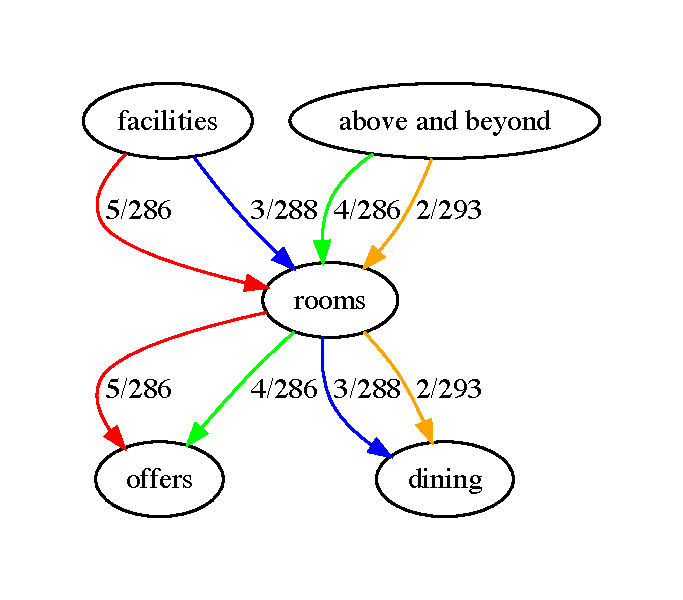
\includegraphics{figs/digraphs/sample_graph}
  \caption[Sample frequency patterns identified in a subset of PC requests]{Sample frequency patterns identified in a subset of PC requests. Refer to Table~\ref{tbl:sample_graph} for frequency pattern interactions.}
  \label{fig:sample_graph}
\end{figure}

\newpage

\subsection{IP Request Sources}

\subsubsection{Internal Site Visitors}

\dotfigure{internal_requests}{Directional network graph visualising frequency patterns of internal visitors made on an internal IP range}

\subsubsection{External Site Visitors}

\dotfigure{external_requests}{Directional network graph visualising frequency patterns of external visitors made on a non-internal IP range}

\subsection{Top Three Countries}

\subsubsection{Hong Kong Visitors}

\dotfigure{hk_requests}{Directional network graph visualising frequency patterns of visitors from Hong Kong}

\subsubsection{USA Visitors}

\dotfigure{us_requests}{Directional network graph visualising frequency patterns of visitors from the United States}

\subsubsection{Australian Visitors}

\dotfigure{au_requests}{Directional network graph visualising frequency patterns of visitors from Australia}

\subsection{Platform Categories}

\subsubsection{PC Visitors}

\dotfigure{pc_requests}{Directional network graph visualising frequency patterns of requests made by PCs}

\subsubsection{Smartphone Visitors}

\dotfigure{smartphone_requests}{Directional network graph visualising frequency patterns of requests made on smartphones}

\subsubsection{Tablet Visitors}

\dotfigure{tablet_requests}{Directional network graph visualising frequency patterns of requests made on tablets}

\subsubsection{Bots Visitors}

\dotfigure{bots_requests}{Directional network graph visualising frequency patterns of requests made by bots}

\newpage
\appendix

\section{Additional Tables}

Below are tables of frequency pattern results for each section identified in Section~\ref{sec:results}.

\csvtable{internal_requests}{Internal Request Frequency Patterns}
\csvtable{external_requests}{External Request Frequency Patterns}
\csvtable{hk_requests}{Hong Kong Frequency Patterns}
\csvtable{us_requests}{USA Request Frequency Patterns}
\csvtable{au_requests}{Australian Request Frequency Patterns}
\csvtable{pc_requests}{PC Request Frequency Patterns}
\csvtable{tablet_requests}{Tablet Request Frequency Patterns}
\csvtable{smartphone_requests}{Smartphone Request Frequency Patterns}
\csvtable{bots_requests}{Bots Request Frequency Patterns}

\clearpage

\section{Web Log Data Format}
\label{apx:data_format}

\section{Extrapolation Results}
\label{apx:results}

Attached on the following pages are the results from Databricks. You may also interact with this online on \href{https://databricks-prod-cloudfront.cloud.databricks.com/public/4027ec902e239c93eaaa8714f173bcfc/7364378259770565/3552971541306612/8155742302574378/latest.html}{Databricks}.


\end{document}
